\documentclass[dutch]{hu}
\usepackage{apa}
\usepackage{natbib}
\usepackage{makecell}
\usepackage{longtable}
\usepackage{makeidx}
\usepackage{pdfpages}
\usepackage{hyperref}
\usepackage{graphicx}
\usepackage{pdflscape}
\date{19 januari 2016}
% \addbibresource{literatuur.bib}
\makeindex
\title{TH06}

\author{Christiaan}{van den Berg}{1660475}
\author{Aydin}{Biber}{1666849}
\author{Martijn}{van Dijk}{1660713}
\author{Chiel}{Douwes}{1666311}

\teacher{Wouter}{van Ooijen}
\teacher{Joost}{Schalken}
\teacher{Marten}{Wensink}
\teacher{Jan}{Zuurbier}
\subtitle{Technisch Verslag}
\begin{document}

\maketitle

\tableofcontents{}

\chapter{Management Samenvatting}
\section{Inleiding}
Samenvatting technisch verslag
\newpage

\section{Code}
Bla Bla code

\subsection{functie() uitleg}
Bla Bla over deze specifieke code
\chapter{Inleiding}
% - Wie heeft om de uitvoering van de opdracht gevraagd (de opdrachtgever)?
% - Wat is de aanleiding voor de opdracht? Waarom wil de opdrachtgever dit?
% - Wie gaan de resultaten van de opdracht gebruiken (de eindgebruikers)?

Er is door de Hogeschool Utrecht opdracht gegeven voor de ontwikkeling van een wasmachine die via een netwerkverbinding te bedienen is. Steeds meer apparaten hebben een internetverbinding, en zijn verbonden met andere apparaten. \cite{wonenTussen100Sensoren}

De opdracht betreft het ontwikkelen van een prototype om in een kleine groep testers te evalueren wat de meerwaarde is van een wasmachine met internetverbinding is. 
\chapter{Onderzoek}
Om dit project te kunnen maken is er onderzoek naar diversen onderwerpen nodig. Zonder dit onderzoek mist er veel informatie die er later in het project nodig zijn om problemen te verhelpen of het project sneller te laten lopen.
OHiervoor zijn de volgende onderwerpen die wij gaan onderzoeken.
\section {Read/Write met RTOS}
Om bij te houden waar het systeem was na stroomuitval is het nodig om de informatie op te slaan in een log bestand, maar omdat het maken en schrijven in een 
bestand een actie van het OS is, kan dit het rest van het systeem in een sleep zetten. Om te onderzoeken of dit een probleem wordt met deadlines van het realtime systeem gaan wij 
onderzoeken hoe lang het duurt om een log file te maken, en dan meerdere keren het bestand openen, schrijven en daarna sluiten om te kijken hoe lang het duurt. Als deze periode niet de 
deadlines overschrijd dan kunnen wij dit gebruiken in het systeem.

\section{Wasprogrammas}
Om te zorgen dat er door specialisten wasprogrammas kunnen worden toegevoegd, moeten wij ons meer verdiepen in hoe de wasprogrammas in elkaar zitten en hoe de 
wasmachine precies werkt, dit wordt vooral veel opzoeken en zelf met een werkende wasmachine uittesten om te kijken hoe de programmas in elkaar zitten.

\section{Snelheid van de UI}
Wij moeten onderzoeken hoe snel het systeem kan reageren op een actie in de UI, zoals de wasmachine stoppen, starten, etc. dit kunnen wij doen door simpelweg te 
kijken naar het systeem nadat wij een bepaalde optie selecteren. 


\chapter{Requirements Architecture}
\section{Use-case diagram}
In dit onderdeel zal het use-case diagram worden gepresenteert en de use-cases worden beschreven.
Wanneer er wordt gerefereerd naar een "gebruiker" dan wordt hiermee de klant bedoelt die de wasmachine gekocht heeft en deze gebruikt om de was mee te doen.
Een "beheerder" is iemand die werkt voor het bedrijf die wasmachine's levert en beheert.

\scalebox{0.7} {
	\includegraphics{Chapters/usage1.png}
}

\section{Use-case beschrijvingen}

	\subsection{Systeem configureren}
	\begin{center}
	  \begin{tabular}{ | p{4cm} | p{8.5cm} | }    \hline
		Doel & Het aanpassen van de pincode of veranderen wat er gebeurt na het uitvallen van de wasmachine. \\ \hline
		Pre-condities & De gebruiker is ingelogd op de webinterface. \\ \hline
		Post-condities & De aangepaste instellingen zijn opgeslagen. \\ \hline
		Uitzonderingen & \\
		\hline
	  \end{tabular}
	\end{center}

	\subsection{De was doen}
	\begin{center}
	  \begin{tabular}{ | p{4cm} | p{8.5cm} | }    \hline
		Doel & Zorgen dat de was gewassen wordt. \\ \hline
		Pre-condities & De gebruiker is ingelogd op de webinterface. \\ \hline
		Post-condities & De wasmachine is een wastaak aan het uitvoeren. \\ \hline
		Uitzonderingen & \\
		\hline
	  \end{tabular}
	\end{center}

	\subsection{Authenticeren}
	\begin{center}
	  \begin{tabular}{ | p{4cm} | p{8.5cm} | } \hline
	  Doel & Vaststellen dat degene die probeert toegang te krijgen tot de webinterface daadwerkelijk bevoegd is om de wasmachine te bedienen. \\ \hline
	  Pre-condities & Er is een webinterface-sessie gestart.\\ \hline
	  Post-condities & De gebruiker is geauthenticeerd. \\ \hline
	  Uitzonderingen & De gebruiker sluit de browser. De wasmachine gaat verder met taken indien deze voor het sluiten waren doorgegeven. \\
	  \end{tabular}
	\end{center}

	\subsection{Software updaten}
	\begin{center}
	  \begin{tabular}{ | p{4cm} | p{8.5cm} | }    \hline
		Doel & Het ontvangen van een update door deze te accepteren. \\ \hline
		Pre-condities & De gebruiker is ingelogd op de webinterface. \\ \hline
		Post-condities & Een nieuw wasprogramma is toegevoegd aan de lijst van wasprogramma's. \\ \hline
		Uitzonderingen &  \\
		\hline
	  \end{tabular}
	\end{center}

	\subsection{Log inzien}
	\begin{center}
	  \begin{tabular}{ | p{4cm} | p{8.5cm} | }    \hline
		Doel & Het lezen van het logbestand om informatie te kunnen achterhalen over het systeem. \\ \hline
		Pre-condities & \\ \hline
		Post-condities & \\ \hline
		Uitzonderingen &  \\
		\hline
	  \end{tabular}
	\end{center}

	\subsection{Hervatten wasprogramma}
	\begin{center}
	  \begin{tabular}{ | p{4cm} | p{8.5cm} | }    \hline
		Doel & Het hervatten van het huidige wasprogramma na een stroomstoring. \\ \hline
		Pre-condities & Er is een stroomstoring geweest waardoor het systeem tijdelijk niet in staat was om het wasprogramma uit te voeren. \\ \hline
		Post-condities & Het systeem is bezit met het uitvoeren van het wasprogramma vanaf het laatst bereikte punt. \\ \hline
		Uitzonderingen & De gebruiker heeft bij de instellingen aangegeven niet het programma te willen hervatten na een storing maar dat deze moet worden stopgezet. Het systeem pompt het water weg en ontgrendelt de deur. \\
		\hline
	  \end{tabular}
	\end{center}
\chapter{Chapter}
\section{Solution Architecture}
Uitleg over het hoofdstuk

\section{Beschrijving architectuur}


\section{Klassendiagram}


\section{Taakstructurering}
taken die zijn onderscheiden
onderbouwing van eventuele samenvoeging van taken
onderbouwing van de periode van periodieke taken
onderbouwing van de deadlnes van taken
motivering voot de gekozen prioriteiten

\newpage
	\begin{landscape}
		\section{Concurrency Model}
		\thispagestyle{empty}

		\includegraphics{Concurrencydiagram1.png}
		Onderbouwing voor de keuzes van synchronisatiemidelen
		Alternatieven die mogelijk zijn
	\end{landscape}

\newpage
	\section{Dynamic model}
		\section{Update Controller}
		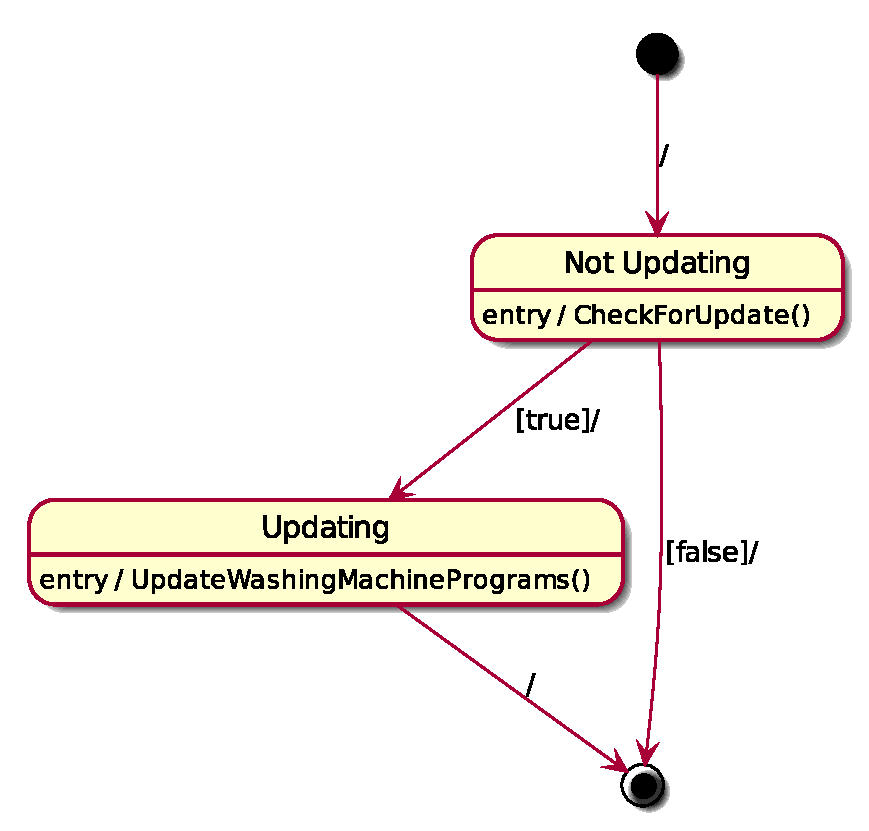
\includegraphics[scale=0.4]{update_controller.eps}

		\section{Authentication Controller}
		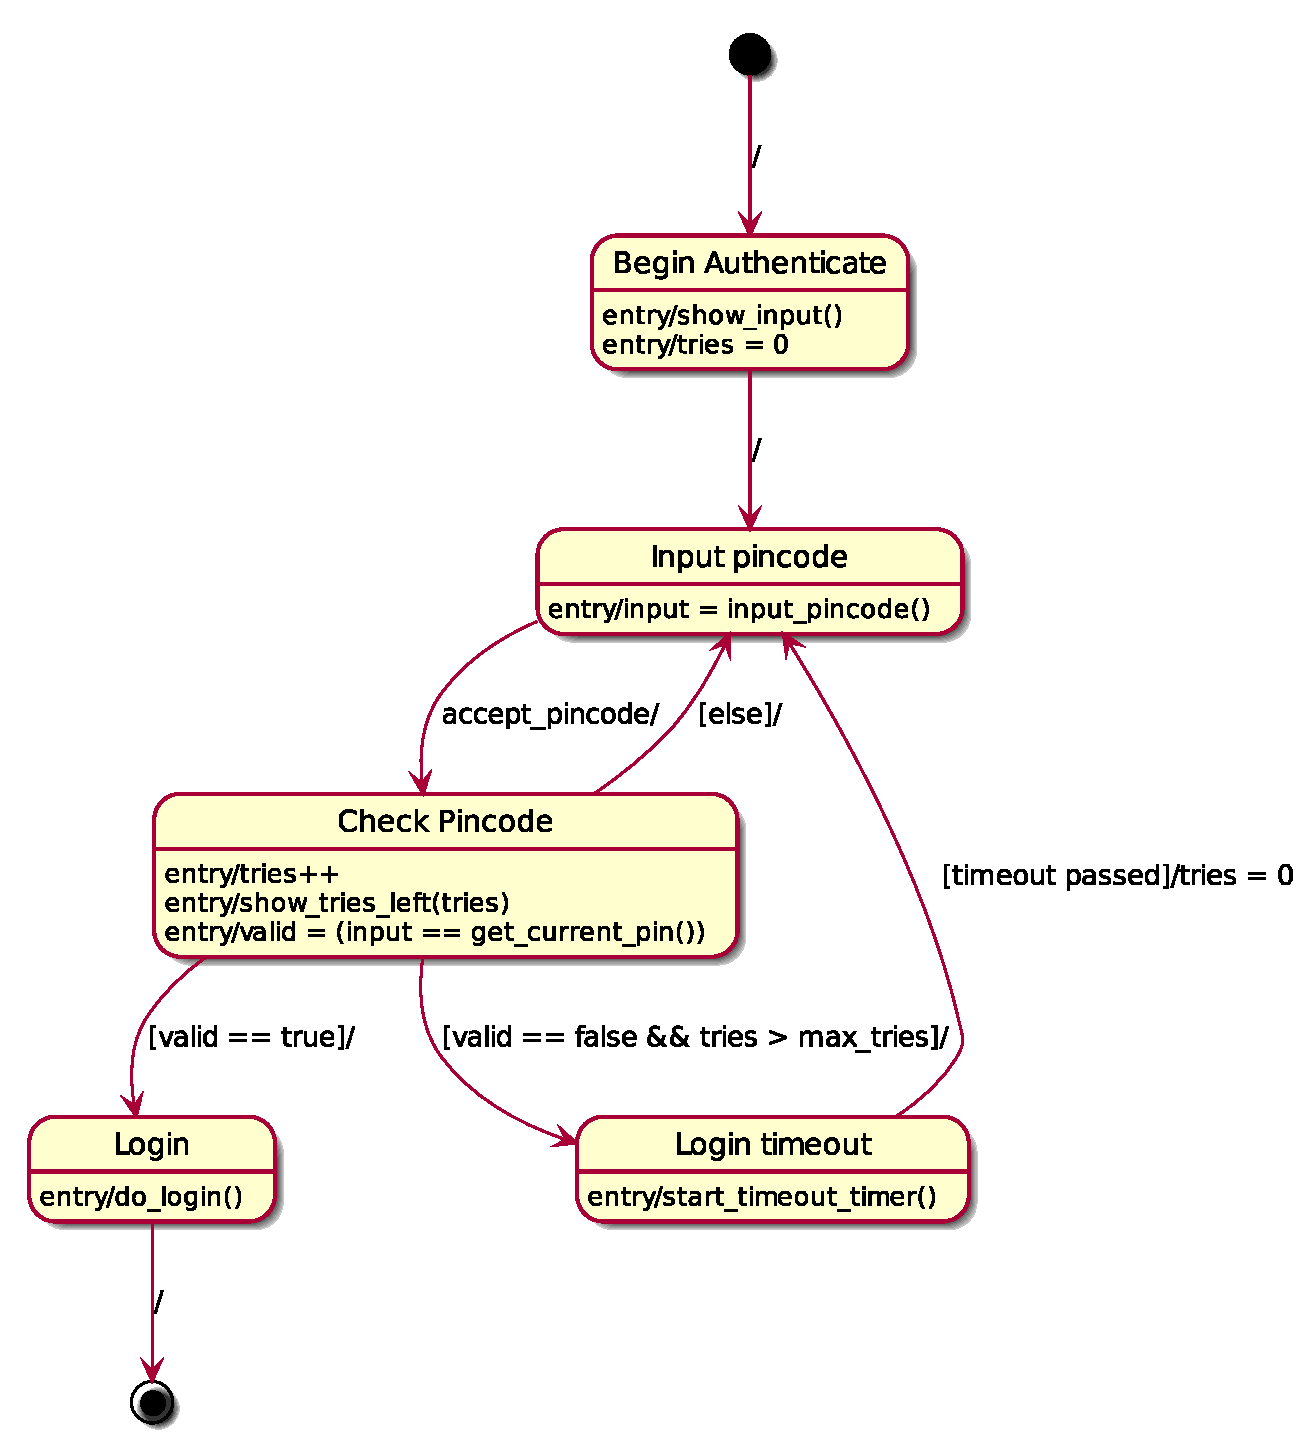
\includegraphics[scale=0.4]{authentication_controller.eps}

		\section{Log Controller}
		\includegraphics[scale=0.4]{log_controller.eps}

		\section{Washing Controller}
		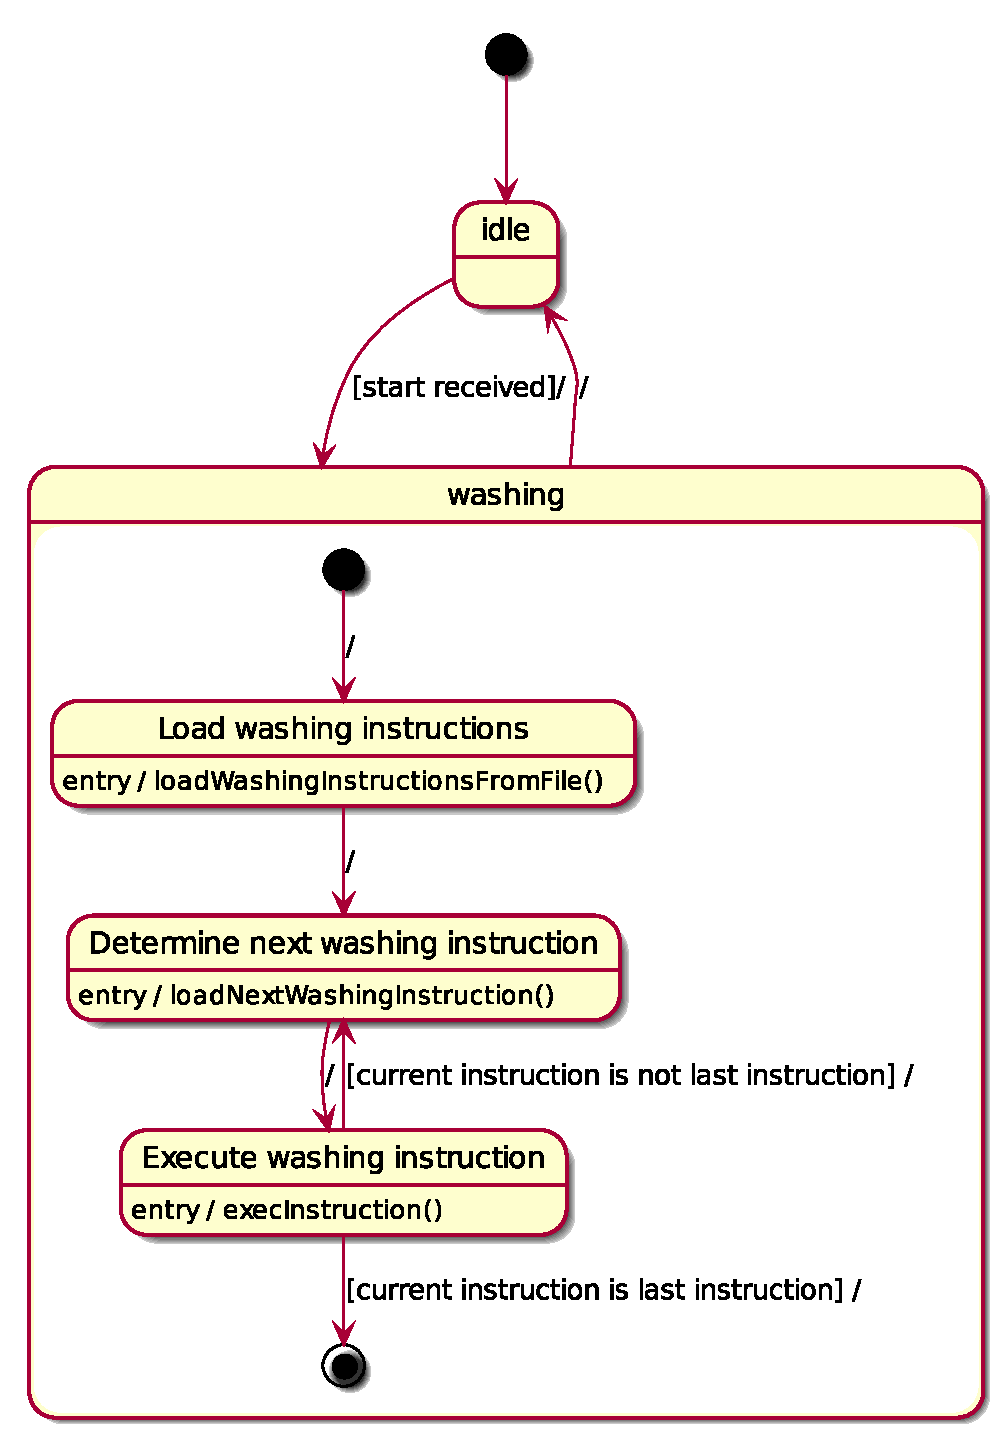
\includegraphics[scale=0.4]{washing_controller.eps}

		\begin{landscape}
			\thispagestyle{empty}
			\section{Settings Controller}
			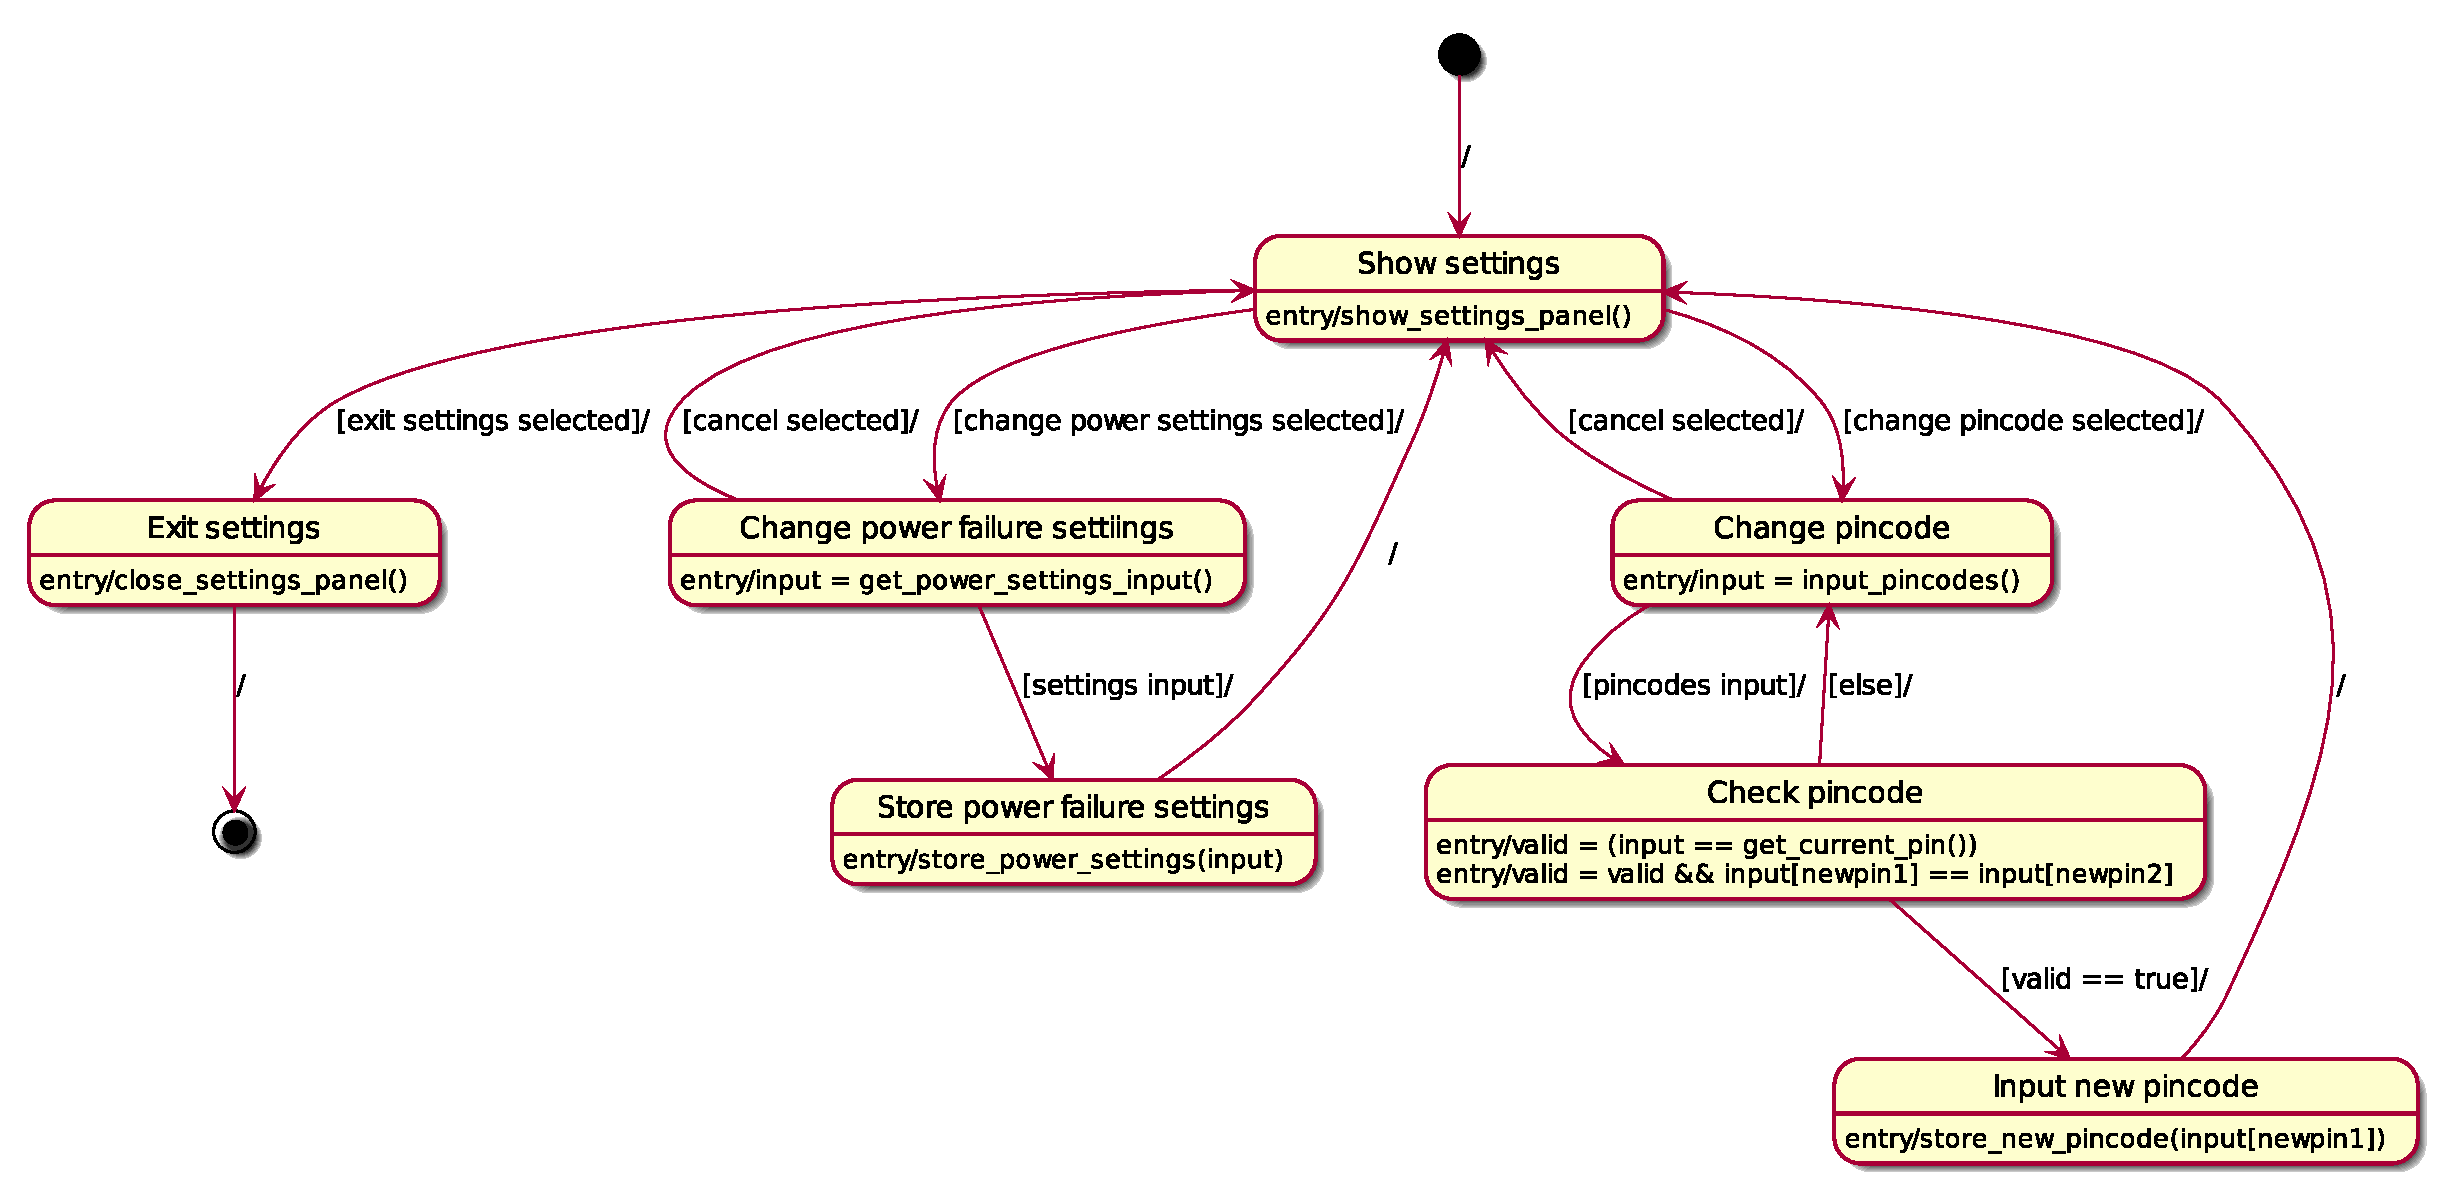
\includegraphics[scale=0.5]{settings_controller.eps}
		\end{landscape}

\section{Communicatie protocol}


\section{Bijlagen}

\chapter{Chapter}
\section{Realisatie}
\newpage

\section{Opgetreden problemen en oplossingen}
Opgetrede problemen

\section{Onopgeloste problemen}
Onopgeloste problemen

\section{Gedetailleerde uitleg code}
int i = 0; houdt in dat een integer genaamd "i" wordt geinstantieerd met een waarde van 0.

\section{Uitgevoerde tests en resultaten}

\chapter{Evaluatie}
\section{Inleiding}
In dit hoofdstuk bespreken wij de onderdelen van de realisatie die achteraf beter hadden kunnen zijn opgelost.
Tevens bieden wij voor deze problemen beter oplossingen die zo gewenst in de toekomst alsnog toegepast kunnen worden.

\section{Communicatie tussen RTOS en de rest van het systeem}
Tijdens de ontwikkeling kwamen wij erachter dat communicatie tussen het RTOS en andere threads vrij omslachtig is. Mogelijk hadden wij dit beter kunnen oplossen door de websocket thread inkomende verbindingen te laten accepteren en de socket objecten vanuit het RTOS op te halen, en deze sockets binnen het RTOS verder af te handelen.


\printbibliography

\end{document}